Im vorherigen Kapitel wurde bereits untersucht wie Projekt- und Projekt-Portfolio-management insbesondere in Kombination mit agiler Methodik die Erreichung strategischer Unternehmensziele unterstützen kann. Durch die regelmäßig anstehenden Entscheidungen besteht der Bedarf für regelmäßiges und vollständiges Reporting, welches für die Entscheidungen herangezogen werden kann, um diese zu objektivieren. In diesem Kapitel soll insbesondere die Automatisierung quantitativer Metriken mit Tools untersucht werden, um Schlüsse für die Umsetzung der Fortschrittsmessung in dieser Arbeit zu ziehen.

\subsection{Reporting für agiles Portfoliomanagement}
Studien zeigten bereits eine positive Korrelation zwischen erfolgreichem Portfoliomanagement und sogenannter Project Portfolio Control (PPC). PPC wird durch drei Faktoren charakterisiert: Projektauswahl, Reporting und Stil der Entscheidungsfindung \cite{ProjectPortfolioControl}.
% Project Portfolio Control and Portfolio Management Performance P.39
% Project Portfolio Control and Portfolio Management Performance P.38
Für die optimale Projektauswahl in PPC wurde bereits untersucht, dass die Entscheidungsfindung optimiert werden kann, indem die Metriken aus dem Reporting, welche für die Entscheidungsfindunge herangezogen werden, mithilfe eines fuzzy Analytic Hierarchy Process (AHP) für eine Priorisierung einzelner Elemente des Portfolios gewichtet werden und anschließen mit der fuzzy TOPSIS Methode in eine Reihenfolge gebracht werden \cite{Mohammed2021}.
% The optimal project selection in portfolio management using fuzzy multi-criteria decision- making methodology P.13
Hieraus lässt sich ableiten, dass es keine generalisierbaren Metriken gibt, die für alle Unternehmen und Projekte gelten, sondern dass die Metriken für jedes Unternehmen und jedes Projekt individuell bestimmt werden müssen. Im Optimalfall sollten also grundsätzlich alle bzw. möglichst viele  Metriken erhoben werden, um sie anschließend zu gewichten.

\subsection{qualitatives vs. quantitatives Reporting}
C. J. Settina und L. Schoemaker \cite{reportingInAgilePortfoliomanagement} untersuchten bereits das Reporting für agiles Portfoliomanagement in einer Fallstudie in mehreren Unternehmen. Aus der Befragung der teilnehmenden Unternehmen ergaben sich folgende Metriken, welche für das Reporting erhoben wurden:

\vspace{20pt}
\begin{center}
  \begin{minipage}{1\linewidth}
    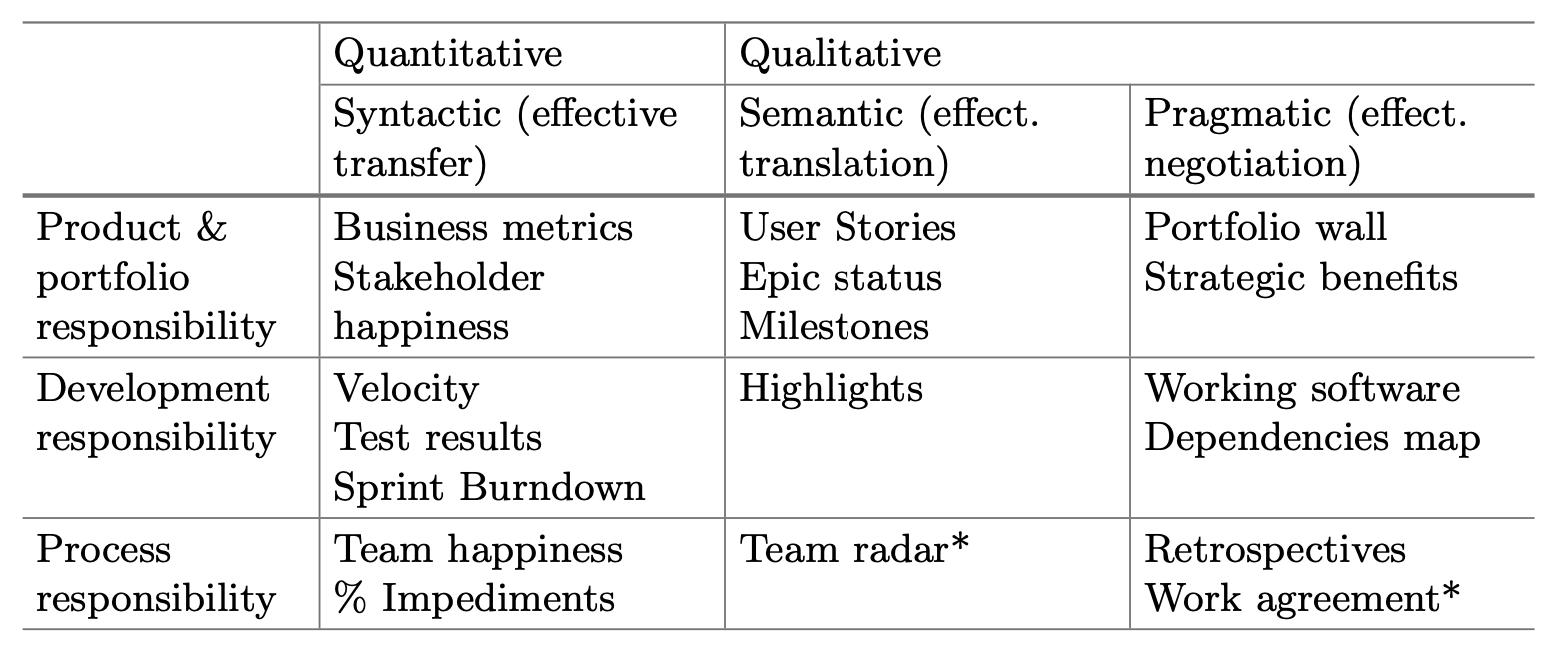
\includegraphics[width=\linewidth]{TableSettinaSchoemaker.png}
    \captionof{figure}{qualitatives und quantitatives Reporting \cite{reportingInAgilePortfoliomanagement} }
  \end{minipage}
\end{center}
\vspace{20pt}


Sie stellten fest, dass für effektives Reporting verschiedene Metriken erhoben werden müssen, welche allgemein in qualitativem und quantitativem Reporting unterteilt werden können.
Qualitatives Reporting zeigt Chancen auf und bietet Kontext, während quantitatives Reporting das Quantifizieren von Elementen und Fortschritt sowie die Validierung von Zielen und geschaffenem Wert ermöglicht.
% Settina und Schoemaker P.212
Aus den gegebenen Metriken kann abgeleitet werden, dass Fortschritt als quantitative Metrik eingeordnet werden kann, da sie vergleichbar mit z. B. Sprint-Burndowns sind, welche letztendlich den Fortschritt über Zeit widerspiegeln.

% \subsection{Reports für Value based Software-Engineering}
% Value-based Software-Engineering(VBSE) ist eine Sammlung von Frameworks für die Entscheidungsfindung in der Softwareentwicklung. VBSE basiert auf der Annahme, dass die Entscheidungen in der Softwareentwicklung auf Basis von einem Kriterium, welches als Wert bezeichnet wird, getroffen werden sollten \cite{}.
% Wert kann hier auf verschiedene Arten definiert werden und kann in mehrere Teile heruntergebrochen werden. Beispiele für Wert sind:
% \begin{itemize}
%   \item Nutzen
%   \item Kosten
%   \item Risiko
%   \item Wert für den Kunden
%   \item Wert für das Unternehmen.
% \end{itemize}

% Unter der Berücksichtigung des Werts können Entscheidungen wertezentiert getroffen werden. Diese Entscheidungen verteilen sich über den gesamten Software-Engineering-Prozess, welcher auch  als VBSE Agenda bezeichnet wird \cite{}.
% Der Prozess kann folgende Teile beinhalten:
% \begin{itemize}
%   \item Requirements Engineering
%   \item Architecting
%   \item Design und Entwicklung
%   \item Verifizierung und Validation
%   \item Planung und Kontrolle
%   \item Risikomanagement
%   \item Qualitätsmanagement
%   \item Mitarbeitermanagement
% \end{itemize}

% \subsection{Teamkoordination}
% Teamkoordination ist ein wichtiger Bestandteil in jeder Form von Projektplanung und -durchführung. In agilen Unternehmen ist Teamkoordination besonders wichtig, da die Teams selbstorganisiert sind und somit die Koordination der Teams untereinander nicht von einer zentralen Instanz übernommen wird und ebenfalls die Projektverantwortung in das Team gegeben wird \cite{}34.
% Somit wird eine gute Teamkoordination kritisch für den Erfolg des Projekts \cite{}.

\subsection{Automatisches Reporting}
Ein weiterer Schluss aus der Arbeit von C. J. Settina und L. Schoemaker \cite{reportingInAgilePortfoliomanagement} ist, dass es sich beim Reporting meist um einen manuellen Prozess handelt, welcher mit wiederkehrendem Aufwand verbunden ist, da die Metriken regelmäßig erhoben werden müssen. Um diesen Prozess des Reportings zu optimieren, sollten qualitative und quantitative Reports unterschiedlich betrachtet werden.

Quantitative Metriken sind quantifizierbar, sodass der Prozess der Erhebung dieser Metriken bei vollständiger Dokumentation aller relevanter Daten automatisierbar ist. Werden diese Metriken dann automatisch erhoben sorgt dies für konsistente, regelmäßige, valide und aktuelle Ergebnissen.

Qualitative Metriken sind dagegen schwer automatisierbar, da sie häufig nicht auf objektiv erfassbaren Daten beruhen. Zur Optimierung kann eine systematische Herangehensweise für die Bestimmung der Metriken definiert werden, um mit deren Hilfe  mehr Konsistenz und Regelmäßigkeit zu gewährleisten. Des Weiteren stellen Sie in ihrer Arbeit die Hypothese auf, dass künstliche Intelligenz in Zukunft eingesetzt werden kann, um auch qualitative Metriken weitestgehend zu automatisieren.
% Settina und Schoemaker P.213

\subsection{Reporting mit digitalen Tools}
Automatisiertes Reporting setzt einen Tool-getriebenen Planungsprozess voraus, um Daten in einem verarbeitbaren Zustand für die Automatisierung zur Verfügung stellen zu können.

\subsubsection{Verwendung von digitalen Tools}
Eine Fallstudie, die mit mehreren IT-Unternehmen durchgeführt wurde, welche aktiv Projekt-Portfoliomanagement betreiben, gibt Empfehlung für eine erfolgreiche Implementierung von Projekt-Portfoliomanagement \cite{guidelinesForPortfoliomanagement}.
Eine dieser Empfehlungen ist die Verwendung eines Systems zur einheitlichen und aktuellen Dokumentation der planungsrelevanten Daten, mit der Reports, die Managemententscheidungen unterstützen, erzeugt werden können.
V. Freitas et al. führten eine weitere Fallstudie durch, die untersuchte wie die Verwendung von webbasierten Tools, speziell dem hier verwendeten ``VALUE''-Tool, Entscheidungsprozesse unterstützen kann \cite{Value-Based-Decision-Making-Case-Study}. Die Ergebnisse zeigten, dass durch die Verwendung des Tools die Entscheidungsfindung und die Qualität der Entscheidungen durch systematische Herangehensweise verbessert wurde.
% V. Freitas, M. Kemppainen, E, Mendes and P. Rodr ́ıguez, “A systematic literature review of value-based decision-making tools,” Submitted to Information and Software Technology.

\subsubsection{Weitere Tools}
Ein vergleichbares Tool zu dem Konzept, welches in dieser Arbeit entwickelt wird, stellt das ebenfalls webbasierte ``Kanbanize'' dar. Es soll ebenfalls Planungselemente in verschiedenen Ebenen miteinander verknüpfen können. Diese Verknüpfungen werden über sogenannte Workflows realisiert, die Abhängigkeiten abbilden können, und dabei sehr spezifisch konfiguriert werden. Dies lässt komplexere Abhängigkeiten als einfache Verknüpfungen zu, erfordert allerdings komplexere Konfigurationen. ``Kanbanize'' stellt sich dabei als All-In-One-Lösung dar und setzt die ausschließliche Verwendung des Tools auch für die operative Arbeit mit Aufgaben voraus, da es keine Synchronisation mit anderen Tools zulässt. Zusätzlich beschränkt sich ``Kanbanize'' auf die Verwendung von Kanban-Boards. Es erlaubt außerdem sehr detaillierte Konfigurationen für das Reporting/Auswerten der aktuell dokumentierten Daten.
